\documentclass{article}

\usepackage{fullpage}
\usepackage{url}
\usepackage{graphicx}
\usepackage{perpage} 
\usepackage{array}
\usepackage{tabularx}

\MakePerPage{footnote} 

\author{Darshan Hegde \\
Center for Data Science \\
New York University \\
e-mail: \texttt{darshan.hegde@cims.nyu.edu}
}
\title{\textbf{Efficient Theano 1D Convolutions for Variable Length Sequences} \\
 Final Report
}
\date{\today}

\begin{document}

\maketitle

\begin{table}[!th]
\begin{tabular}{l p{0.8\textwidth}}
Supervisor & Prof. Georg Stadler \\
Course &  MATH-GA 2012.003 High Performance Computing \\
\end{tabular}
\end{table}

\begin{abstract}
In this repost, we motivate the need for efficient 1D convolution kernels that support variable length sequences for Theano. Then we provide details of implementation and optimizations. At last, we compare our implementation with Theano's default implementation with zero padding.   
\end{abstract}

\section*{Motivation}
Convolution Networks are used heavily used by Computer Vision Researcher and has outperformed other conventional techniques on many important benchmark tasks \cite{ImageNet}. Theano \cite{Theano-2012} \cite{bergstra+al:2010-scipy} is mathematical expressions compiler library which can efficiently compile both CPU and GPU codes. Many Computer Vision researchers have been using Theano \cite{Theano-2012} \cite{bergstra+al:2010-scipy} for building and experimenting with Convolution Networks and has very efficient implementation of 2D convolutions on GPU. Since one needs to evaluate (and take gradients of weights w.r.t cost function) Convolution Networks on a large number of training images (usually color with 3 channels) during training of the network, 2D convolution is implemented as 4D tensor operation with input represented as (images-per-batch, channels, width, height) and output represented as 4D tensor (images-per-batch, num-conv-kernels, out-width, out-height). On a typical GPU implementation, training images are processed in mini-batches and each image in a given mini-batch is processed in parallel. All images in a given training dataset are of same size (height and width) and hence amount of computation done per image are uniform.

Recently, Natural Language Processing (NLP) researchers have applied Convolution Networks for tasks such as Sentiment Analysis \cite{KalchbrennerACL2014} and Document Summarization \cite{Denil2014c} with state of the art performance. Convolution operation used in NLP are applied on 1D variable length sequences (Sentence is a sequence of words / Document is sequence of sentences). One can use efficient 2D convolutions in Theano to compute 1D convolutions by setting one of the dimensions (height or width) to 1. However, to compute 1D convolutions for sentences in a mini-batch (just like we do for images) one needs to use zero-padding for shorter sentences. Using this strategy,  width of a given mini-batch is decided by longest sentence and for shorter sentence we are wasting many computation cycles where there is zero-padding. This effect of wasting computations due to zero-padding is quite significant in NLP because sentence are of varying lengths. Fig \ref{fig:sent_lens} shows distribution of sentence lengths in Trip Advisor Hotel Reviews Dataset. This motivates us to implement a separate 1D convolution kernel for Theano which avoids zero-padding for variable length sequences. 

 \begin{figure}[!htbp]
\begin{center}
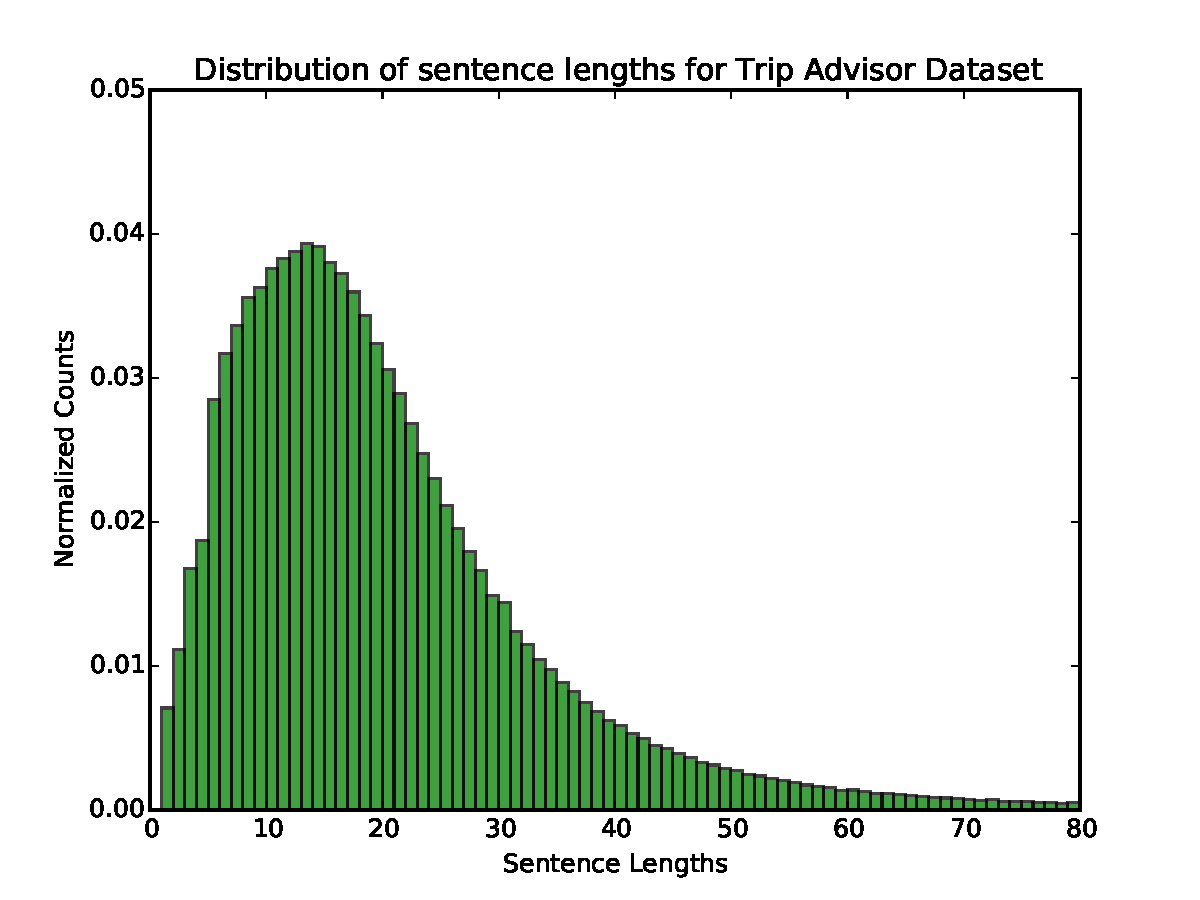
\includegraphics[scale=0.4]{sentence_len_dist.pdf}
\end{center}
\caption{Distribution of sentence lengths in Trip Advisor Dataset}
\label{fig:sent_lens}
\end{figure}

\section*{Implementation Details}
 Fig \ref{fig:convnet} shows Convolution Network used for modeling a document. One typically applied multiple convolution filters in each layer to extract different features. Convolution operation in each layer is called full convolution and is given by following formula,
 \[  
 OUT^n[i, k] = \sum_{j = max(0, i-w_k+1)}^{min(i, l_n-1)} \sum_d IN^n_{(j, d)} \circ KERN_{(w-1-i+j, d)}^k
 \]
Where $n$ is the sentence index, $i$ is the output location index, $k$ is the kernel index, $j$ is the running index of where convolution is applied,  $d$ is the index for dimension of the input.  $OUT^n[i, k]$ indicates output value for $n^{th}$ sentence at output location $i$ and kernel $k$, $IN^n_{(j, d)}$ is the input value for $n^{th}$ sentence at input location $j$ and dimension $d$ and $KERN_{(w-1-i+j, d)}^k$ is kernel value for $k^{th}$ kernel at location $w-1-i+j$ and dimension $d$. $w_k$ is width of $k^{th}$ convolution kernel.

So the formula suggest that serial computation involves 5 loops one for each index $n$ sentence index, $i$ output index, $k$ kernel index, $j$ input index and $d$ dimension index. 

 \begin{figure}[!htbp]
\begin{center}
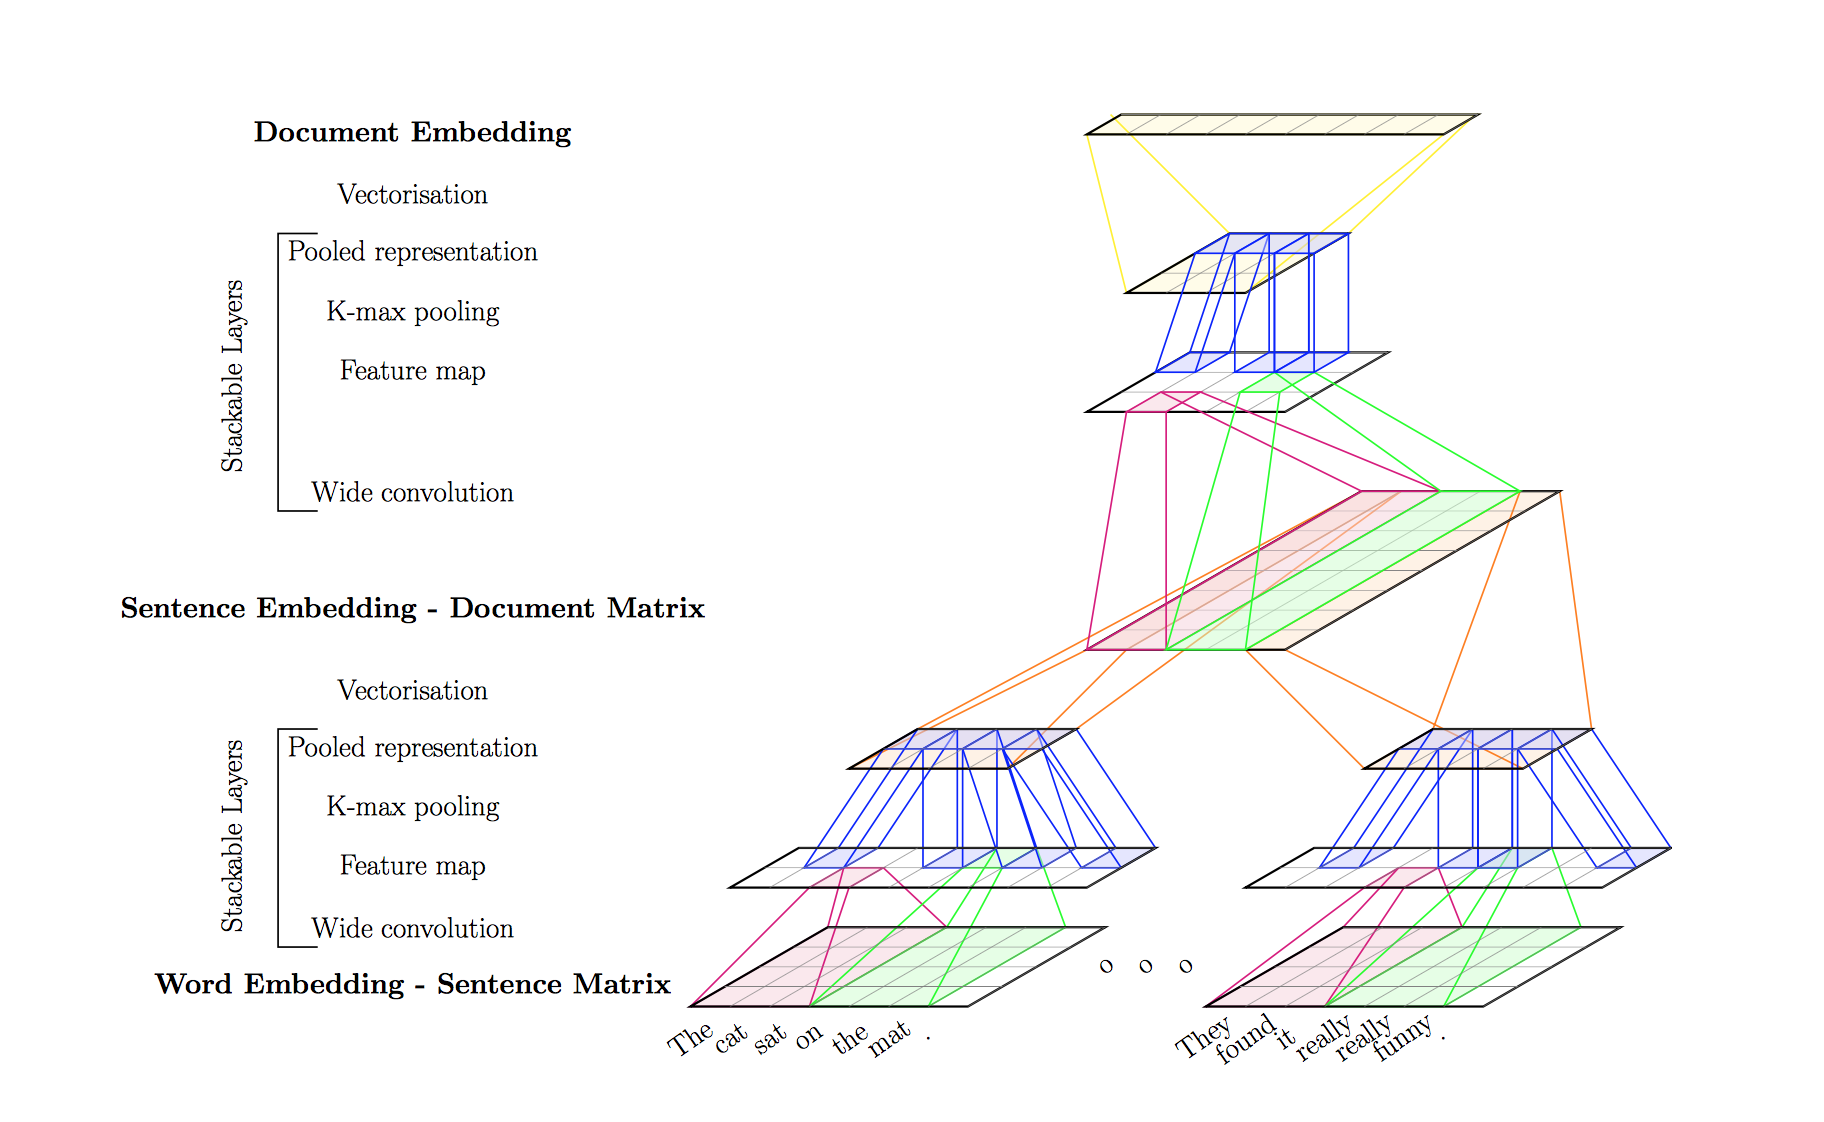
\includegraphics[scale=0.35]{document_model.png}
\end{center}
\caption{Convolution Network Architecture for Document Modeling. Picture courtesy: Denil et. al. \cite{Denil2014c} }
\label{fig:convnet}
\end{figure}

We choose to implement 1D convolutions using CUDA because Theano library uses CUDA as it's backed for 2D convolutions and many other operations and already has interfaces for integrating CUDA code. From here on we assume that the reader is familiar with CUDA API and it's terminology. An important design decision to be made before writing CUDA kernels is to decide what each block computes and what each thread computes. 

Since $n$ is the index for sentence and is the largest index, it's natural to assign it to a block. So each block computes convolutions on a given sentence. But now, each block has variable length of convolutions to compute which calls for some for load balancing in a mini-batch. CUDA run-time takes care of scheduling blocks such that resource requirements are met and each multi-processor is utilized to maximum extent. Hence, by assigning each variable length sequence to a block we have mitigated the load balancing to CUDA runtime. Within each block, for high performance CUDA requires that each thread performs same computation on different data points. Since in each dimension we are performing element-wise multiplication and summation, we assign each dimension to a thread. 

\section*{Optimizations}

\begin{enumerate}
\item \textbf{Minimum branch divergence}: Each thread in a given block computes the same element-wise product between input and kernels, the CUDA kernel has no branch divergence there. But computing the summation across dimensions ($\sum_d$) in the formula has some branch divergence but that is very minimal too.

\item \textbf{Shared memory summation}: For computing the summation across dimensions ($\sum_d$) in the formula, we store each individual element-wise products in a shared memory to save global memory bandwidth. So for each output location $i$ and kernel $k$ there is just 1 write operation to global memory.

\item \textbf{Global memory coalescing}: Inputs and Kernels are stored in dimension major order. Within the CUDA kernel, each thread in a block accesses consecutive dimensions and hence all the accesses to Inputs and Kernels are global memory coalesced.  

\end{enumerate}

\section*{Experimental Results}
We ran all our run-time comparisons on NVIDIA GRID K520, which has CUDA compute capability of 3. We compare our implementation to Theano's implementation with zero-padding. Obviously, if all the sentences in a given mini-batch are of the same length then Theano's implementation outperforms our implementation because Theano's GPU code has been optimized for over 7 years now. 

For comparing the performance we use the similar set of parameters used in the $1^{st}$ layer of Convolution Network used by Denil et. al. \cite{Denil2014c}. Firstly, we compare the performance for 1d convolution where dimension=100, convolution kernel width=7, mini-batch size=200, number of kernels=64 and batch size=100 with all sentence having the same length=50. We found that Theano's implementation was about \textbf{1.2x} faster than our implementation. 

We use sentence lengths from Trip Advisor Dataset and initialize inputs and kernels randomly for all experiments. We use dimension=100, convolution kernel width=7, mini-batch size=200, number of kernels=64 and batch size=100 held fixed and change the parameter of interest. 
Fig \ref{fig:minibatch} shows the performance of our implementation compared to Theano's implementation with zero padding as we vary mini-batch size parameter. As seen from Fig \ref{fig:minibatch} as we increase the size of the mini-batch, speed up due to our implementation goes up as number of zero-padding increases and thus the amount of not useful computation in Theano's implementation. We want to use larger mini-batches so that convergence of training is smoother. Researcher typically use a mini-batch size of $[100, 500]$, in case of larger mini-batch size $500$ we get upto \textbf{2.6x} speedup. As Fig \ref{fig:n_kerns} and Fig \ref{fig:w_kerns} performance is quite robust to number of kernels and width of kernels. An example of optimization done by Theano is shown in Fig \ref{fig:w_kerns} for width of the kernel = 9. For larger kernel size's Theano's implementation does some optimization to make it run faster. However, typical size of the kernels used by Denil et. al. \cite{Denil2014c} is $\{5, 7\}$ and Computer Vision Researchers have found that smaller kernel sizes and deeper networks work much better. 

Finally, The kernel achieves CGMA (Compute to Global Memory Access ratio ) of $\approx 7.2$.  

 \begin{figure}[!htbp]
\begin{center}
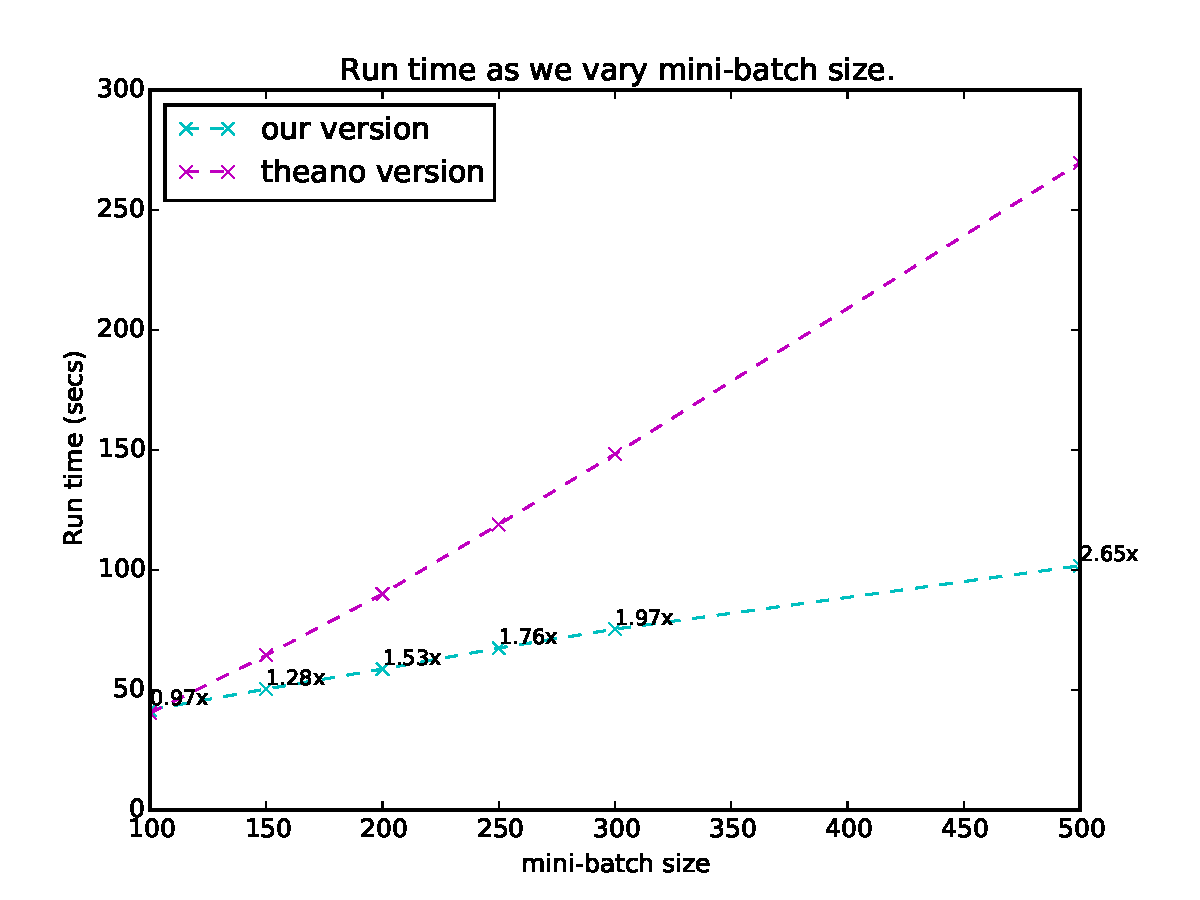
\includegraphics[scale=0.6]{mini-batch.pdf}
\end{center}
\caption{Performance of our implementation as we vary mini-batch size}
\label{fig:minibatch}
\end{figure}

 \begin{figure}[!htbp]
\begin{center}
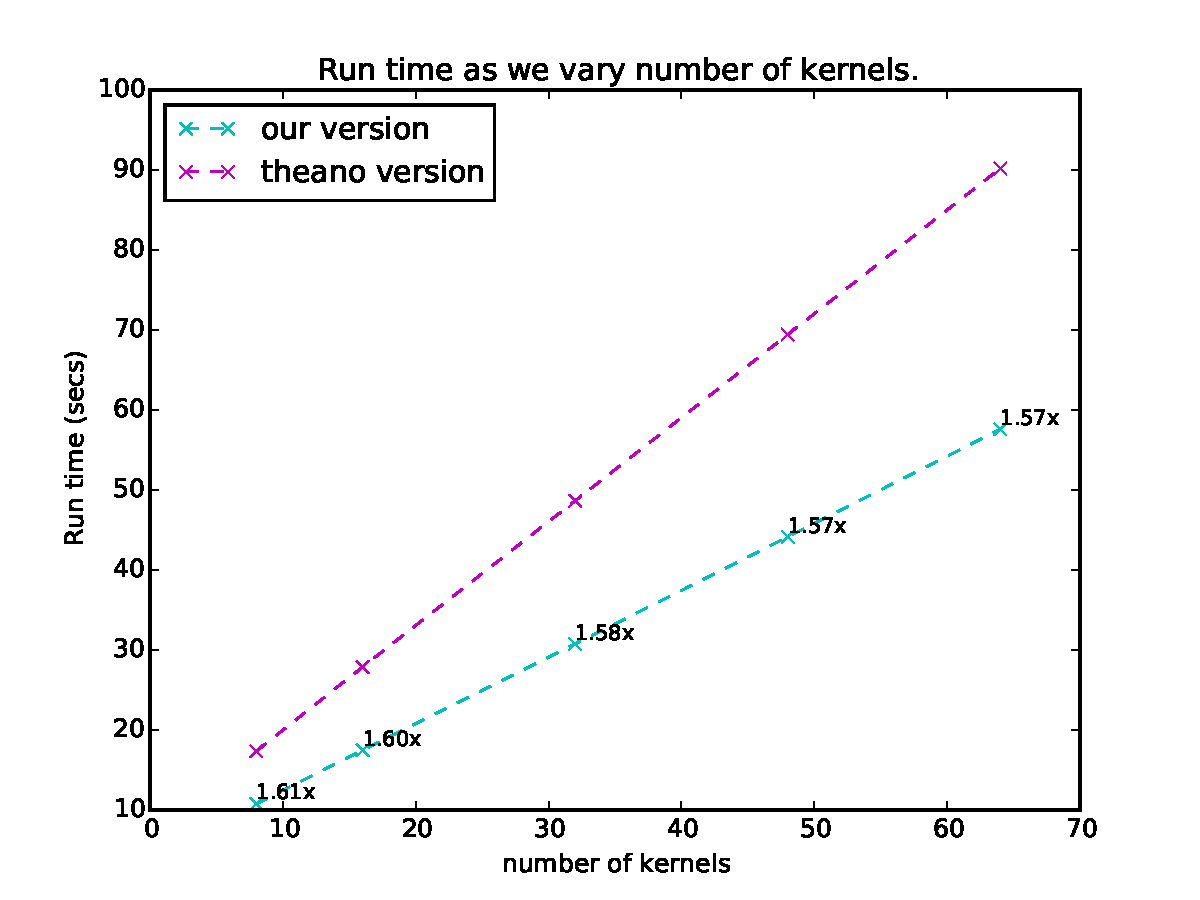
\includegraphics[scale=0.6]{n-kerns.pdf}
\end{center}
\caption{Performance of our implementation as we vary number of kernels}
\label{fig:n_kerns}
\end{figure}

 \begin{figure}[!htbp]
\begin{center}
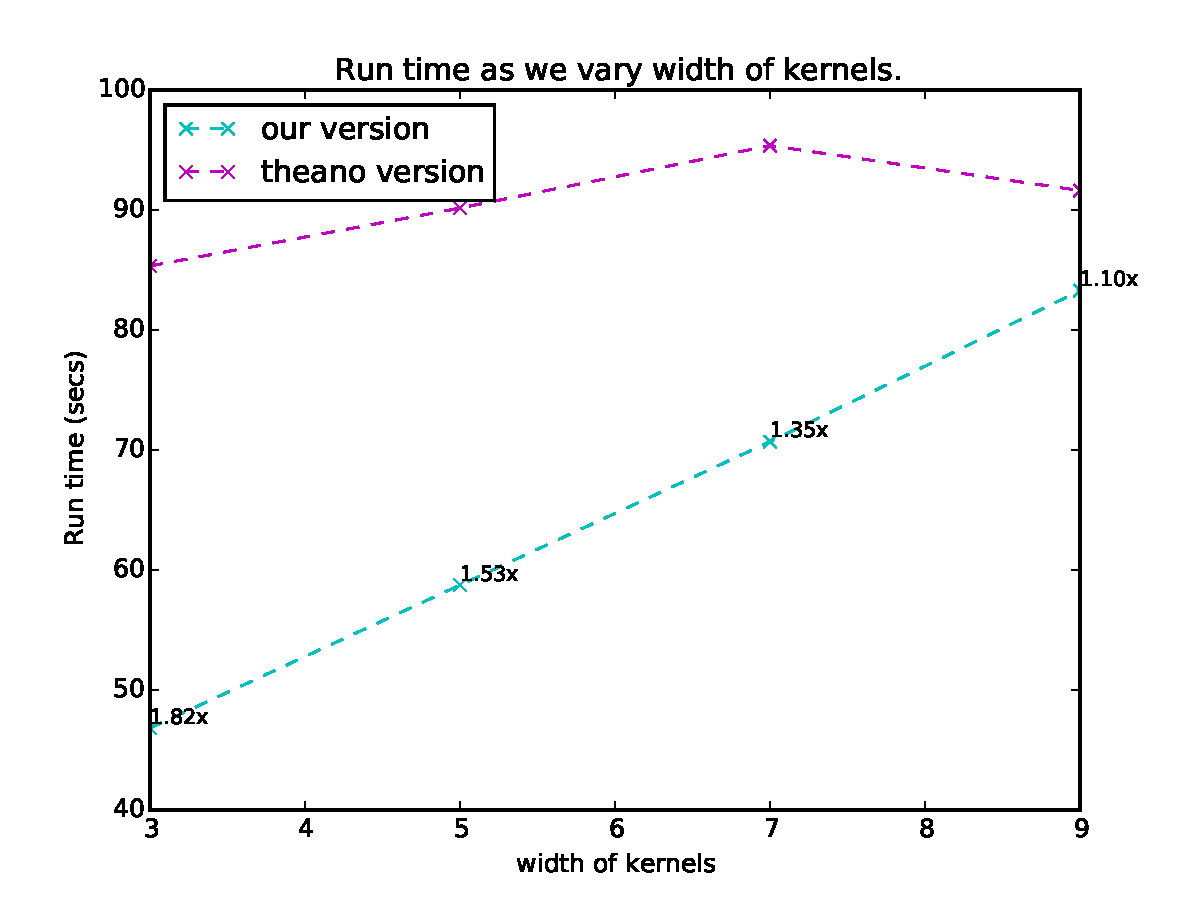
\includegraphics[scale=0.6]{w-kerns.pdf}
\end{center}
\caption{Performance of our implementation as we vary width of kernels}
\label{fig:w_kerns}
\end{figure}
 
\section*{Future Extensions}
 
We plan to optimize our implementation even further so that we match the performance of Theano implementation on sentences of uniform lengths. Also, we need to integrate our implementation with Theano python API and release it for the benefit of larger research community. 

\clearpage

\bibliographystyle{plain}
\bibliography{final_report}

\end{document}

